\chapter{Introducción}
\label{cap:Introduccion}
Actualmente la demanda energética en el planeta no deja de crecer, y para lidiar con ello deben llevarse a cabo medidas para reducir el consumo elevado de energía, lo que se conoce como eficiencia energética. La eficiencia energética~\cite{GarSa12} se refiere al empleo de medios de optimización en la producción y aprovechamiento de la energía, con el objetivo de proteger el medio ambiente. Esto ha pasado a ser una necesidad debido a que las emisiones de $ CO_{2} $ van en aumento y el cambio climático es un hecho.\\

Por otro lado, puesto que las fuentes de energía fósil y nuclear son finitas, podría llegar el día en el que no se pueda satisfacer la demanda energética, salvo que se apueste por los métodos alternativos de obtención de energía. Es aquí donde entran en juego las energías renovables. Una de ellas es la energía solar~\cite{Perp12}, que permite el aprovechamiento de la radiación electromagnética del sol. Resulta interesante su estudio, debido a que es tan abundante que se considera inagotable: la cantidad de energía que el Sol vierte diariamente sobre la Tierra es diez mil veces mayor que la consumida al día en todo el planeta. Finalmente, además de ser una energía inagotable, es una energía limpia, una muy buena alternativa a los combustibles fósiles o energía nuclear. \\

Teniendo en cuenta estos dos antecedentes, existe una motivación a la hora de apostar por medios de extracción de energía renovables y por la eficiencia energética. Actualmente la mayoría de particulares tienen una única fuente de suministro de energía que vendría a ser la compañía eléctrica de la cuál son clientes, importando la totalidad de la energía que su hogar demanda a dicha compañía, a un precio establecido \gls{PVPC}~\cite{Ree14} (Precio voluntario al pequeño consumidor) que representa el precio máximo de referencia que pueden contratar los consumidores con hasta 10 Kwh de potencia contratada. Actualmente existen un gran número de fuentes de extracción de energía cuyos precios y potencia generada varían a lo largo del tiempo, e incluso del día. Estos cambios son dependientes de un gran número de factores. Sería interesante poder reducir la cantidad de energía que se obtiene de esta fuente en las horas pico (horas de máximo consumo donde el \gls{PVPC} suele alcanzar el valor alto) y obtenerla de otra fuente cuyo precio sea menor, para así obtener un promedio mucho mas barato que con una única fuente de energía. Esto puede lograrse añadiendo nuevas fuentes al hogar, como puede ser la instalación de placas fotovoltaicas. Este procedimiento está regulado, pues en el año 2015 mediante el Real Decreto 900/2015~\cite{Boe15} se establecieron unas condiciones para la instalación de placas fotovoltaicas, lo que se conoce coloquialmente como el impuesto al sol. Por suerte, para potencias contratadas no superiores a 10 Kwh, no se pasa este impuesto, así que no es problema para el desarrollo y aplicación del sistema.\\

En este \gls{TFG} se ha decidido enfocar la base de conocimientos adquiridos por el alumno durante el grado para plantear una solución a la problemática anterior. Se propone emplear las ciencias de la computación para optimizar el uso de la energía eléctrica a nivel particular al máximo posible. Para aprovechar al máximo esta situación de manera utópica, una persona dispondría de varias fuentes de obtención y su energía demandada estaría siendo obtenida de la manera más eficiente en cada momento. Lamentablemente este objetivo es ardúa tarea para el ser humano, pero alcanzable para la computación.

Con todo lo expuesto antes, como idea general se puede concluir en que este \gls{TFG} se centrará en la creación de un \textbf{sistema inteligente} para la gestión de energía en el hogar de la manera más óptima y eficiente posible. En función de un escenario determinado en cada hora del día, el sistema será capaz de modelar la cantidad de energía eléctrica recibida por cada una de las fuentes de entrada energética para realizar el menor gasto económico posible en su obtención. De igual modo, deberá modelar la cantidad de energía eléctrica suministrada a una serie de salidas, pues toda la energía generada debe ser consumida de uno u otro modo, como puede ser el consumo del hogar, carga de una batería, etc. Esto se traduce en una optimización y aprovechamiento de la energía, que además tiene como consecuencia un ahorro económico en la obtención de la energía necesaria. En la Figura~\ref{fig:abstract} se muestra un esquema del sistema propuesto donde se identifican desde un alto nivel de abstracción los elementos generadores de energía y los elementos consumidores.\\
\begin{figure}[!h]
	\centering
	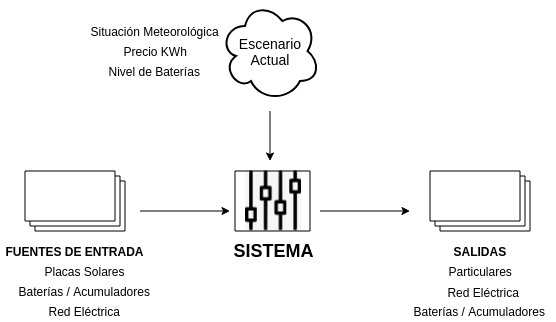
\includegraphics[width=10cm]{figs/Abstract.png}
	\caption{Dibujo del sistema}
        \label{fig:abstract}
\end{figure}

Finalmente, para hacer visual y probable el sistema, se creará una aplicación web en la que los usuarios podrán interactuar. En dicha aplicación se podrá realizar simulaciones de optimización en un día deseado, cuyos resultados serán desglosados y comparados con el gasto real producido ese día, dejando constancia de la utilidad y satisfacción de objetivos que tendrá el sistema. Esta aplicación será alojada en Internet y cualquier persona, con previo registro, podrá usarla.\\

Este documento está formado por los capítulos expuestos a continuación.

\section{Estructura del TFG}
\begin{description}
\item \textbf{~\ref{cap:Introduccion}. Introducción}\\
  Se muestra la problemática inicial, se plantea e introduce este \gls{TFG} como solución y se muestra un esquema abstracto del sistema propuesto.
\item \textbf{~\ref{cap:Objetivo}. Objetivos}\\
  Se plantean y definen tanto el objetivo principal como los objetivos parcialesa desarrollar.
\item \textbf{~\ref{cap:Antecedentes}. Motivación y Antecedentes}\\
  Se muestra el estado del arte y se definen los conceptos de computación mas importantes que se emplean en este proyecto.
\item \textbf{~\ref{cap:Metodologia}. Metodología}\\
  Se muestra y define la metodología de proyecto empleada. Se habla acerca de como ha sido adaptada a este caso particular y se describen las tecnologías y herramientas utilizadas.
\item \textbf{~\ref{cap:Resultados}. Resultados}\\
  Se describen los resultados obtenidos a lo largo del desarrollo del \gls{TFG} desde el inicio hasta el final, siguiendo la metodología definida, poblemas encontrados y soluciones empleadas.
\item \textbf{~\ref{cap:Conclusiones}. Conclusiones}\\
  Se habla acerca de las conclusiones e ideas obtenidas tras finalizar el proyecto y se plantean posibles ampliaciones y trabajo futuro.
\item \textbf{Anexo~\ref{cap:AnexoA}. Caso de optimización}\\
  Se puede consultar un Listado con el resumen de simulación del día 11/04/2019. Esta información concierne al fichero generado al realizar una optimización de ese día.
\item \textbf{Anexo~\ref{cap:AnexoB}. \textit{Tests} del proyecto}\\
  Se explica el framework de \textit{tests} usado para realizar los casos de prueba del proyecto software. Esto es necesario pues garantiza tolerancia a fallos y la demostración de la funcionalidad del sistema.
\end{description}
